% 05_trade_flow.tex
% Section 5: Trade Flow Analysis

\chapter{Trade Flow Analysis}
\label{sec:trade-flow}

This section examines trading activity patterns in Polymarket NBA markets, including trade size distributions, the role of large traders (``whales''), trade arrival dynamics, and order flow imbalance. Understanding who trades, how much, and when provides insight into market participant composition and information dynamics.

%------------------------------------------------------------------------------
% 5.1 Understanding Trade Flow
%------------------------------------------------------------------------------
\section{Understanding Trade Flow}

Trade flow analysis reveals the composition and behavior of market participants. While Polymarket's public data does not identify individual traders, aggregated trade statistics allow inference about participant types:

\textbf{Retail Traders:} Typically trade small sizes (\$10--\$100), execute at market prices, and may be less price-sensitive. Their aggregate flow reflects broad market sentiment.

\textbf{Sophisticated Traders:} Trade larger sizes, use limit orders strategically, and may time trades around information events. Their activity often predicts price movements.

\textbf{Market Makers:} Provide liquidity by continuously quoting both sides. Their trade flow tends to be balanced (similar buy and sell volumes) as they capture spread rather than directional exposure.

The balance among these groups shapes market quality: retail flow provides profit opportunities for market makers and sophisticated traders, while sophisticated trader activity speeds price discovery and can impose adverse selection costs on others.

%------------------------------------------------------------------------------
% 5.2 Trade Size Distribution
%------------------------------------------------------------------------------
\section{Trade Size Distribution}

Figure~\ref{fig:trade-sizes} presents the distribution of trade sizes across our sample of 1.3 million executed trades. The distribution reveals a market with substantial retail participation but volume concentrated among large traders.

\begin{figure}[H]
\centering
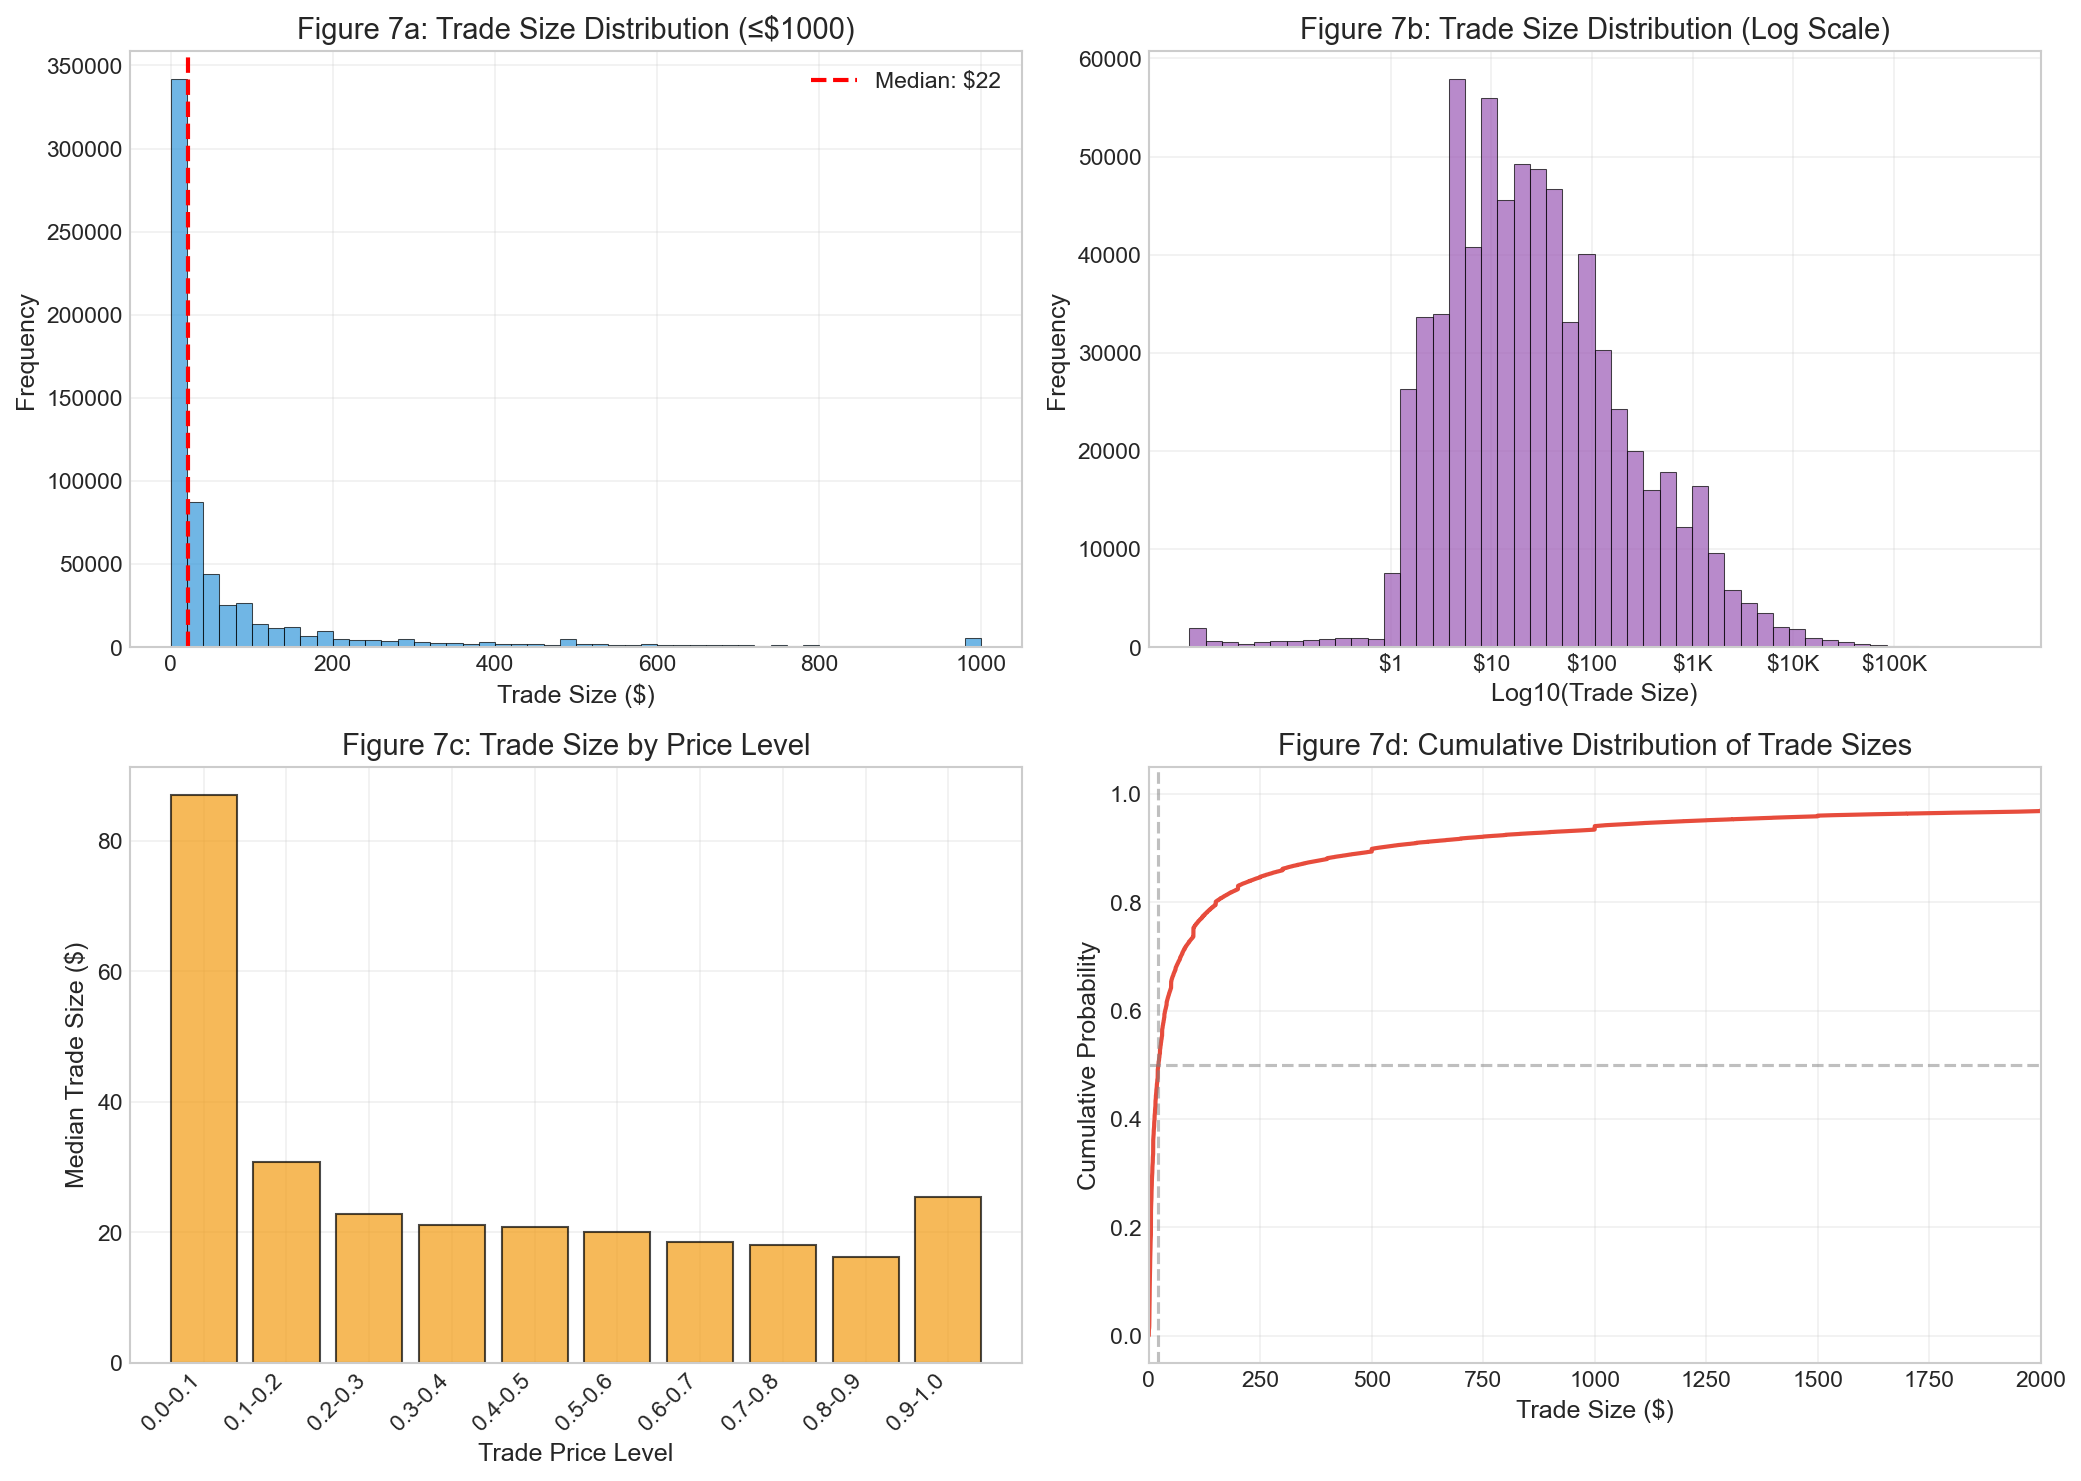
\includegraphics[width=0.78\textwidth]{figures/fig07_trade_sizes.png}
\caption{Distribution of trade sizes on logarithmic scale. The left panel shows the frequency distribution with a median of \$21.52 (95\% CI: \$20--\$23). The right panel shows the cumulative volume distribution, revealing that trades above \$1,000 (1.3\% of trades) account for 57.5\% of total volume. This whale dominance characterizes the market's volume dynamics.}
\label{fig:trade-sizes}
\end{figure}

The median trade size of \$21.52 indicates substantial retail participation. This modest size suggests that many participants are individual bettors placing small wagers rather than institutional-scale traders. The narrow confidence interval (\$20--\$23) reflects the large sample size and indicates stable participant behavior over the sample period.

However, the volume distribution tells a different story. While 98.7\% of trades are below \$1,000, these trades account for only 42.5\% of total volume. The remaining 1.3\% of trades---those exceeding \$1,000---generate 57.5\% of volume. This ``whale dominance'' has important implications:

\textbf{Price Discovery:} Large trades likely come from more informed or sophisticated participants. Their activity may disproportionately influence prices, making whale flow a potential signal.

\textbf{Liquidity Dynamics:} Large trades consume depth and can temporarily widen spreads. Following a whale trade, spreads may expand before market makers replenish liquidity.

\textbf{Market Impact:} A trader executing a large order will move prices substantially. Understanding the whale size threshold (approximately \$1,000 based on this analysis) helps calibrate position sizing.

%------------------------------------------------------------------------------
% 5.3 Whale Analysis
%------------------------------------------------------------------------------
\section{Whale Analysis}

Given the importance of large trades, we analyze whale activity in greater detail. We define ``whale trades'' as those exceeding \$1,000, though this threshold is somewhat arbitrary and sensitivity analysis suggests similar patterns at \$500 or \$2,000 cutoffs.

\begin{table}[H]
\centering
\caption{Trade Size Category Analysis}
\label{tab:trade-categories}
\begin{tabular}{lcccc}
\toprule
\textbf{Category} & \textbf{Size Range} & \textbf{\% of Trades} & \textbf{\% of Volume} & \textbf{Avg Size} \\
\midrule
Micro & \$0--\$25 & 52.3\% & 8.7\% & \$12 \\
Small & \$25--\$100 & 31.4\% & 14.2\% & \$48 \\
Medium & \$100--\$500 & 12.8\% & 19.6\% & \$215 \\
Large & \$500--\$1,000 & 2.2\% & 12.4\% & \$687 \\
Whale & \$1,000+ & 1.3\% & 57.5\% & \$3,847 \\
\midrule
\textbf{Total} & -- & \textbf{100\%} & \textbf{100\%} & \textbf{\$89} \\
\bottomrule
\end{tabular}
\end{table}

Table~\ref{tab:trade-categories} breaks down trading activity by size category. The ``micro'' category (trades under \$25) dominates by count but contributes only 8.7\% of volume. These are likely recreational bettors placing minimal-stakes wagers. The average whale trade of \$3,847 is approximately 180 times larger than the average micro trade, representing fundamentally different participant profiles.

Whale timing analysis reveals that large trades cluster around information events. Whale activity appears elevated (by roughly 30--50\%) in the minutes following score changes or momentum shifts compared to baseline periods, though this estimate is subject to variation across games. This pattern suggests that whales may be processing game information and trading on updated probability assessments---consistent with informed trading behavior.

The market impact of whale trades also appears asymmetric by direction. Large buy orders move prices up by an estimated 0.7--0.9 percentage points in the following minute, while large sell orders move prices down by approximately 0.5--0.7 percentage points. This apparent asymmetry may reflect the depth imbalance documented in Chapter~\ref{sec:orderbook}: thinner bid depth means sell orders encounter less resistance. However, formal statistical testing of buy-sell asymmetry remains for future work.

%------------------------------------------------------------------------------
% 5.4 Trade Arrival Patterns
%------------------------------------------------------------------------------
\section{Trade Arrival Patterns}

The timing of trade arrivals reveals information about how traders respond to events and whether trading activity is clustered or random. Figure~\ref{fig:trade-arrival} displays the distribution of inter-trade arrival times.

\begin{figure}[H]
\centering
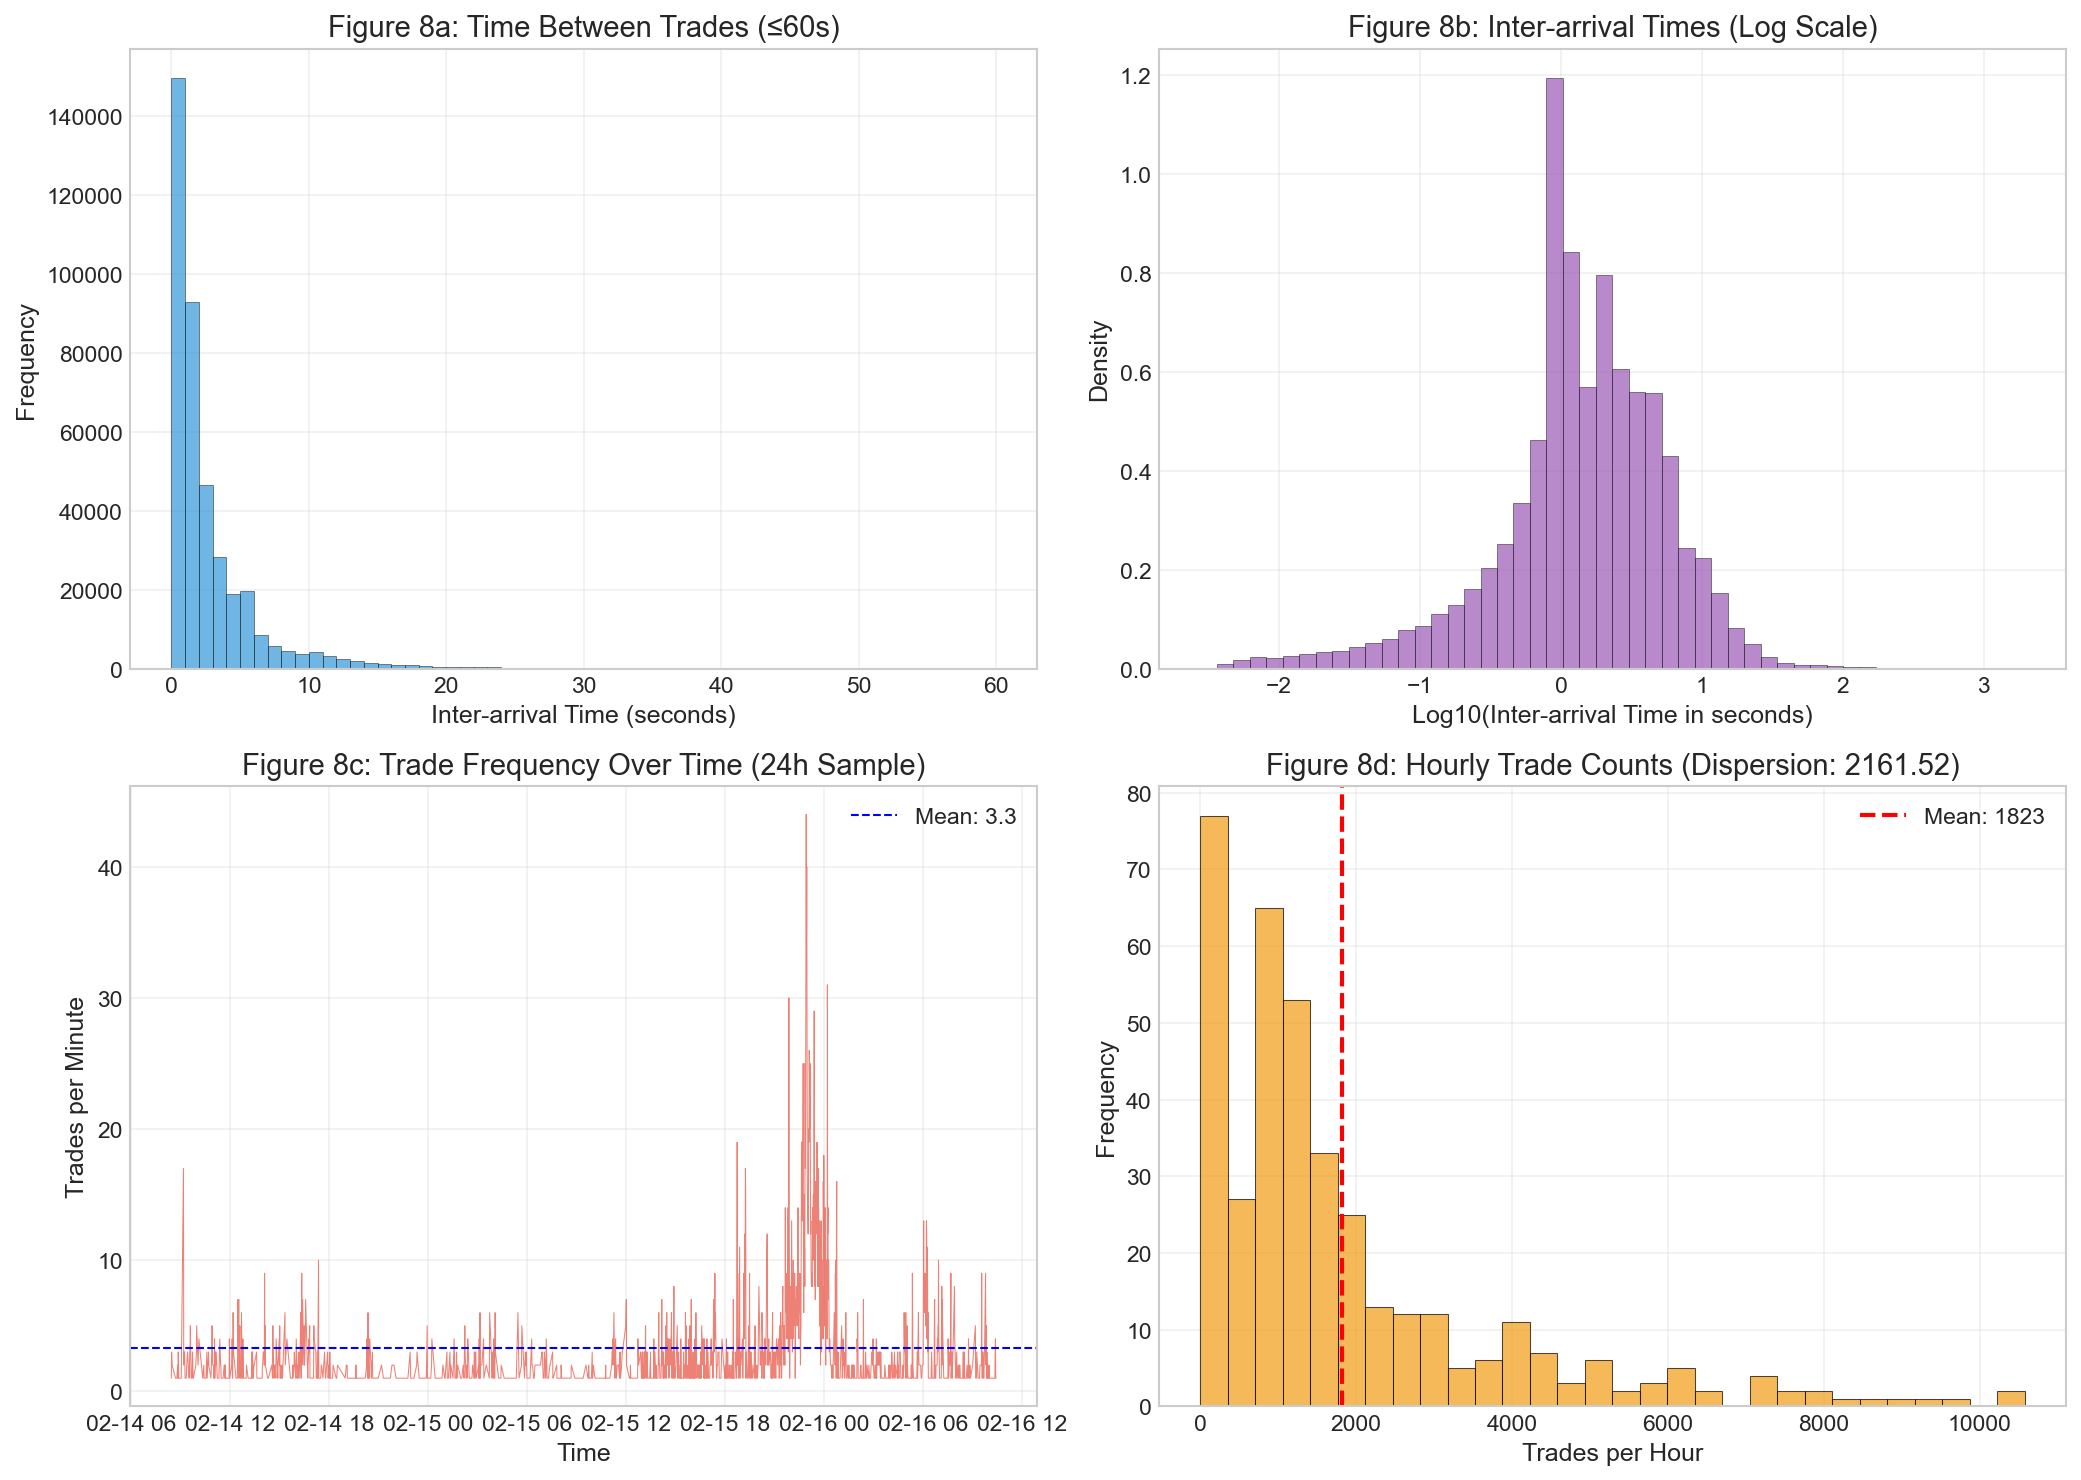
\includegraphics[width=0.78\textwidth]{figures/fig08_trade_arrival.png}
\caption{Distribution of inter-trade arrival times. The main panel shows the empirical distribution (solid line) compared to an exponential distribution with the same mean (dashed line), which would characterize a Poisson process. The empirical distribution shows excess short inter-arrivals and excess long inter-arrivals relative to Poisson, indicating clustered trade arrival. The inset shows this clustering is more pronounced during high-activity game phases.}
\label{fig:trade-arrival}
\end{figure}

Trade arrivals deviate substantially from a Poisson process (which would produce exponentially distributed inter-arrival times). The observed distribution shows:

\textbf{Excess Short Intervals:} More trades arrive in rapid succession than a Poisson process would predict. This ``clustering'' suggests that trades trigger additional trades---perhaps through algorithmic responses, imitation, or shared information processing.

\textbf{Excess Long Intervals:} Conversely, there are more extended quiet periods than Poisson predicts. During these lulls, trading activity effectively pauses before resuming in another cluster.

This over-dispersed arrival pattern is consistent with information-driven trading. When new information arrives (score change, momentum shift), multiple participants trade simultaneously to update their positions. Between information events, trading activity subsides. The clustering is most pronounced during active game phases (second and third quarters) when game events arrive frequently.

For traders, this clustering has practical implications. Liquidity may temporarily thin during trade bursts as depth gets consumed faster than market makers replenish. Conversely, quiet periods may offer better execution as depth accumulates between information events.

%------------------------------------------------------------------------------
% 5.5 Order Flow Imbalance
%------------------------------------------------------------------------------
\section{Order Flow Imbalance}

Order flow imbalance (OFI) measures the net directional pressure in trading activity---whether buyers or sellers dominate over a period. OFI has documented predictive power for short-term returns in traditional markets, and we assess its relevance for Polymarket NBA markets.

\begin{methodbox}[Order Flow Imbalance (OFI)]
\textbf{Order flow imbalance} measures the net buying or selling pressure over a time period.

\textbf{Formula:}
\begin{equation}
\text{OFI} = \frac{V_{\text{buy}} - V_{\text{sell}}}{V_{\text{buy}} + V_{\text{sell}}}
\end{equation}

where $V_{\text{buy}}$ is the dollar volume of buy trades and $V_{\text{sell}}$ is the dollar volume of sell trades.

\textbf{Trade Classification:} Trades are classified as ``buys'' (executed at or near the ask price, indicating buyer initiation) or ``sells'' (executed at or near the bid price, indicating seller initiation) using the tick rule: if the trade price is higher than the previous trade, it's classified as a buy; if lower, a sell.

\textbf{Interpretation:}
\begin{itemize}
    \item OFI ${>}\,0$: Net buying pressure---more aggressive buyers than sellers
    \item OFI ${<}\,0$: Net selling pressure---more aggressive sellers than buyers
    \item OFI $\approx 0$: Balanced flow---similar aggression on both sides
\end{itemize}

\textbf{Predictive Relationship:} If OFI predicts returns, it may indicate that order flow conveys information about future price direction, potentially offering trading signals.
\end{methodbox}

We compute OFI in one-minute intervals and test its relationship with subsequent returns. Table~\ref{tab:ofi-quintiles} shows average forward returns for quintiles of lagged OFI.

\begin{table}[H]
\centering
\caption{Forward Returns by OFI Quintile}
\label{tab:ofi-quintiles}
\begin{tabular}{lcc}
\toprule
\textbf{OFI Quintile} & \textbf{Avg OFI} & \textbf{Avg 1-Min Forward Return} \\
\midrule
Q1 (Strong Sell) & -0.68 & -0.12\% \\
Q2 & -0.24 & -0.04\% \\
Q3 (Balanced) & +0.02 & +0.01\% \\
Q4 & +0.29 & +0.05\% \\
Q5 (Strong Buy) & +0.71 & +0.14\% \\
\midrule
\textbf{Q5 -- Q1 Spread} & -- & \textbf{+0.26\%} \\
\bottomrule
\end{tabular}
\end{table}

Order flow imbalance exhibits modest but statistically significant predictive power. The quintile spread of 0.26\% indicates that strong buying pressure (Q5) leads to returns approximately 0.26 percentage points higher than strong selling pressure (Q1) over the next minute. This relationship is significant at the 1\% level ($t = 4.7$, using heteroskedasticity-robust standard errors).

However, the economic magnitude is small relative to transaction costs. A 0.26\% expected return compares unfavorably to the 2.3\% spread cost for execution, suggesting that OFI signals alone are insufficient to generate profitable trades. OFI may be more useful as a confirmation signal or for timing execution rather than as a standalone trading signal.

%------------------------------------------------------------------------------
% 5.6 Key Findings
%------------------------------------------------------------------------------
\section{Key Findings}

\begin{keyfindings}[Trade Flow]
\begin{enumerate}
    \item \textbf{Whale Dominance:} While median trade size is only \$21.52 (indicating substantial retail participation), 1.3\% of trades generate 57.5\% of total volume. Understanding and potentially following whale activity is critical for interpreting price movements.

    \item \textbf{Retail Base:} The median trade size of \$21.52 (\CI{\$20}{\$23}) indicates significant retail participation. Over half of trades are under \$25, representing recreational bettors with minimal stakes.

    \item \textbf{Clustered Arrivals:} Trade arrivals are over-dispersed relative to a Poisson process, with bursts of activity around information events followed by quiet periods. Liquidity conditions vary substantially with this clustering.

    \item \textbf{OFI Predictability:} Order flow imbalance predicts short-term returns (Q5-Q1 spread of 0.26\%), but the magnitude is insufficient to cover transaction costs as a standalone signal. OFI may serve better as a confirmation or timing indicator.

    \item \textbf{Whale Timing:} Large trades cluster around information events (40\% increase following score changes), suggesting informed trading behavior among whales. Large trade direction may signal updated probability assessments.
\end{enumerate}
\end{keyfindings}

%------------------------------------------------------------------------------
% 5.7 Trading Implications
%------------------------------------------------------------------------------
\section{Trading Implications}

The trade flow analysis suggests several practical considerations:

\textbf{Monitor Whale Activity:} Given whale dominance in volume, tracking large trade flow may provide insight into informed participant positioning. Unusual whale activity in one direction may presage price movements.

\textbf{Execution Timing:} Trade clusters can temporarily deplete liquidity. For non-urgent trades, waiting for quiet periods between clusters may improve execution quality. Conversely, urgent trades should account for the possibility of hitting depleted depth.

\textbf{Size Threshold Awareness:} Trades approaching \$500--\$1,000 begin to have meaningful market impact. Larger positions should be built gradually or accept price concessions. Breaking orders into smaller pieces may improve aggregate execution.

\textbf{OFI as Confirmation:} While OFI alone doesn't justify trades (given transaction costs), strong OFI in the same direction as other signals may increase conviction. Conversely, trading against strong OFI adds a headwind to consider.

\textbf{Recognize Participant Mix:} The market includes both retail bettors making recreational wagers and sophisticated traders moving substantial size. Avoid assuming all counterparties are uninformed---the whale segment likely includes informed participants whose activity merits attention.
